% Created 2018-01-09 Tue 09:05
% Intended LaTeX compiler: pdflatex
\documentclass[a4paper,oneside]{article}
\usepackage[utf8]{inputenc}
\usepackage[T1]{fontenc}
\usepackage{graphicx}
\usepackage{grffile}
\usepackage{longtable}
\usepackage{wrapfig}
\usepackage{rotating}
\usepackage[normalem]{ulem}
\usepackage{amsmath}
\usepackage{textcomp}
\usepackage{amssymb}
\usepackage{capt-of}
\usepackage{hyperref}
\hypersetup{colorlinks=true,linkcolor=blue}
\setcounter{secnumdepth}{4}
\author{Santhanaraj Chellaiah}
\date{Jan 8, 2018}
\title{Cycle Time Reduction of D-301 Blender}
\hypersetup{
 pdfauthor={Santhanaraj Chellaiah},
 pdftitle={Cycle Time Reduction of D-301 Blender},
 pdfkeywords={Cycle time, process optimization, instrumentation, controller, NC-701, unit based control},
 pdfsubject={},
 pdfcreator={Emacs 27.0.50 (Org mode 9.1.6)}, 
 pdflang={English}}
\begin{document}

\maketitle
\begin{abstract}
The D-301 blender is the one that blends NC-701 with different
products to produce various required compositions. NC-701 is unloaded
from a truck to the blender manually and the blending process is
intiated. This however has limited the availability of blender to a
point where the blender can be used only if the truck is available,
thus increasing the cycle time for an output from D-301. This paper
proposes the introduction of a buffer storage tank D-12516 along with
piping, valves, pumps and other instrumentation to reduce the cycle
time of the D-301 blender.
\end{abstract}

\section{Keywords}
\label{sec:org91d40d8}
\emph{Cycle time, process optimization, instrumentation, controller, NC-701, unit based control}

\section{Introduction}
\label{sec:orgfad5b0c}
It is proposed that the material (NC-701) from the truck be unloaded
to a buffer storage tank D-12516. D-12516 will serve as a holding tank
when the trucks are available to unload. The material can be
transferred from D-12516 to D-301 as and when required. Material
unloading from the truck will be effected by pump MP-516T. This pump
could either transfer the material to D-12516 or to D-301
directly. The material stored in D-12516 can be transferred to D-301
using MP-516A pump.  

The following are the two benefits that are expected out of this proposal: 
\begin{itemize}
\item The cycle time of D-301 will be greatly reduced
\item The truck waiting times can be drastically reduced resulting in lower cost
\item The product stored in D-12516 can be stored and maintained at a
temperature, most suited for blending
\end{itemize}
\section{Overall Scheme}
\label{sec:org905994b}
Below is the overall scheme for the project. 
\begin{figure}[htbp]
\centering
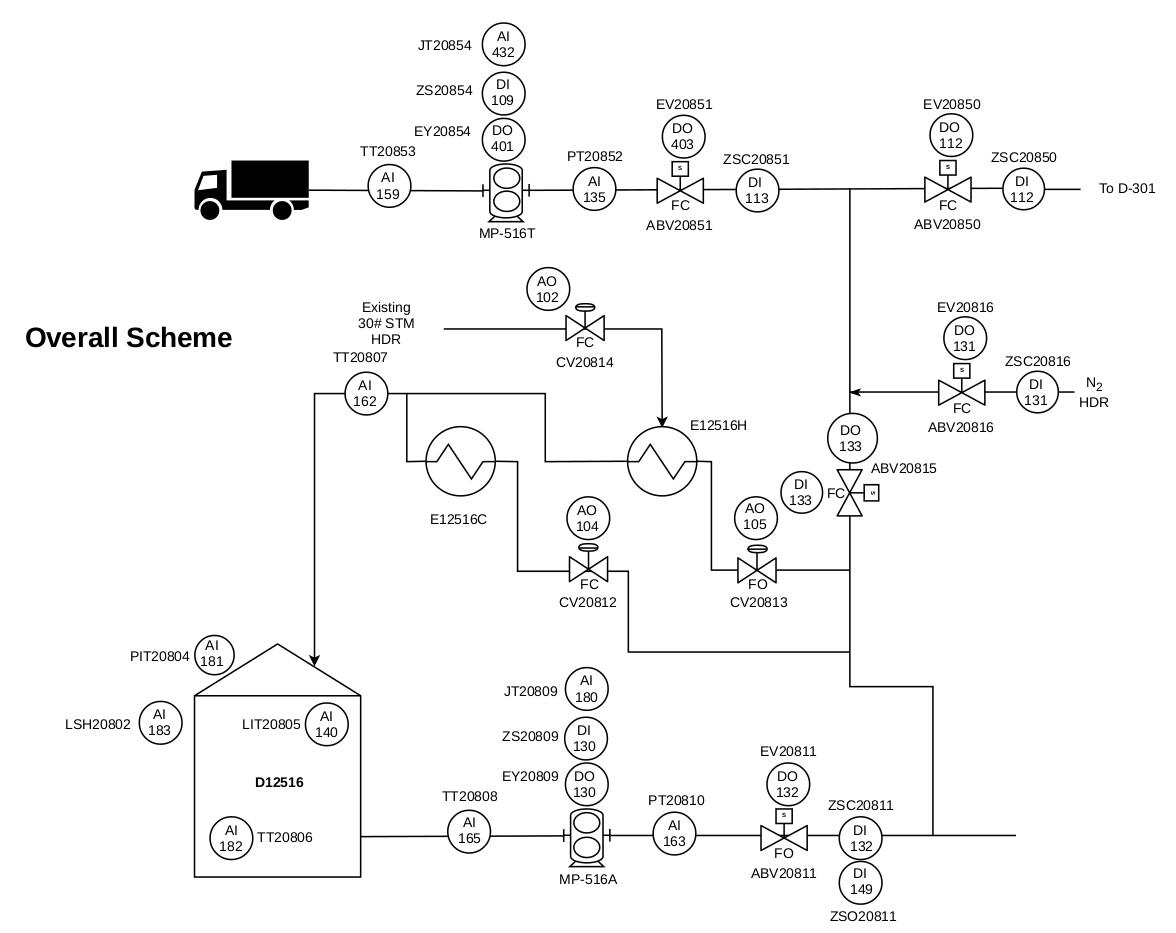
\includegraphics[angle=90,width=10cm]{/home/prasanna/Documents/git/CSR/images/Overall_Scheme.png}
\caption{Schematic showing truck unloading, D-12516 tank and path to D-301}
\end{figure}

\section{Process Narrative}
\label{sec:org79730ff}
The addition of a buffer storage tank calls for a operating procedure
to unload from the truck, recycle the product (and regulate
temperature, if required) and transfer to D-301 when required. It
should also specify when a direct transfer from tank truck can be
initiated toward the blender D-301. The following section details the
process narrative using state based (or unit based control). :width 15cm
\subsection{State based control}
\label{sec:orgb89fb59}
The following is the abstract from the white paper presented by David
A.Huffman on benefits of State Based Control.
\begin{quote}
State Based Control is a plant automation control design based on the
principle that all process facilities operate in recognized, definable
Process States that represent a variety of normal and abnormal
conditions of the process. State Based Control, implemented with the
latest developments in object-based technologies, delivers direct
benefits to its adopters in a variety of Operational Excellence
categories. It results in productivity increases, higher asset
utilization of both people and process, automated responses and
recovery for abnormal conditions and provides an environment for
knowledge capture directly into the control design.
\end{quote}
The proposal intends leverage the State Based Control scheme for this
implementation. The various steps involved in control and operation of
the plant are listed below: 
\begin{enumerate}
\item Maintenance Wait
\item Process Wait
\item Recycle
\item Transfer
\item Unload
\item Direct Transfer
\item Line Clear
\end{enumerate}
\subsection{Steps}
\label{sec:orgaf623c8}
\subsubsection{Maintenance Wait}
\label{sec:org83bdb9b}
In this step, the instruments and the control system are in
maintenance. 

All the process valves will assume thier safe state. The
outputs from the control sytem will be in Fail-safe state. All (or
most) of the instruments are in de-energized state. Most of (or all
non-critical) the alarms are disabled in this step.
\subsubsection{Process Wait}
\label{sec:orge884d51}
This is the step in which all the instruments, valves and the control
system remain energized. The plant is preparing for start up. 

The maintenance/operation team should ensure that all (or almost all)
instruments and valves are in healthy condition. Most of the alarms
are enabled in this step. Maintenance/operation would look of
instrument out of service alarms. If any of the devices are in
"out-of-service" state, they should be fixed and put in service for a
effect a start up.
\subsubsection{Recycle}
\label{sec:orgb3153de}
During the recycle step, the temperature of the product can be
controlled, if required. NC-701 is ideal for blending when its
temperature is around 45 degree Celcius. NC-701 is a highly viscous
liquid which needs to be agitated periodically to maintain consistency
of the product.

During the winter months, the product temperature drops because of
ambient tempertuare. In order to compensate and supplement heat to the
product, NC-701 can be passed through a heat exchanger in order to
raise its temperature. The NC-701 would pass through the tube side of
the exchanger. The shell side would pass a 30 barg steam from the
plants' existing steam header. The flow rate of NC-701 through the
heat exchanger E-12516H can be effected by throttling the control
valve CV-20813. If the product temperature drops, the steam control
valve CV-20814 should approach 100\% open position while the CV-20813
should approach around 50\% of opening. The best ratio of opening the
steam line vs opening the NC-701 line should be ascertained during
operation / trail run for utmost efficiency

During the summer months, the product temperature could go way beyond
the desired setpoint and might require cooling before being
blended. For this case, we can close CV-20813 and also the steam valve
CV-20814 and let the NC-701 to recycle through CV-20812. The tube side
of the exchanger E-12516C would pass NC-701. The shell side would pass
the cooling tower water to effect cooling of NC-701. The flow rate of
NC-701 is adjusted using the control valve CV-20812 to effect the
desired cooling. Note that, the cooling tower water does not have any
controls on it which is unlike the steam control line which is used in
the heating circuit.
\subsubsection{Transfer}
\label{sec:orga16f2fb}
During this step, the material from D-12516 will be transferred to
D-301 blender. 

The pump MP-516A will be used to effect this transfer via the ON-OFF
valves EV-20811, ABV-20815 and ABV-20850. During the transfer step, it
should also be ensured that the control valves CV-20812 and CV-20813
remain completely closed to avoid any recirculation. The nitrogen
purge line should also remain isolated (or closed) using EV-20816.
Before a transfer is initiated, sufficient level in D-12516 must be
ensured. This will prevent the dry running of MP-516A which might in
turn damage the seal of the pump. D-12516 should be at least at 60\%
level (arbitrary value) to intiate a transfer.
\subsubsection{Unload}
\label{sec:orgc378cc2}
During the unload step, NC-701 is unloaded from the truck to
D-12516. 

The pump MP-516T is utilized to pump the material from the truck to
the tank. Since unloading requires manual connection of the unload
hose to the tank truck, a signal to indicate ready-to-unload is
provided by the operator. This signal will serve as a permissive to
starting MP-516T pump. The material will flow via the pump MP-516T,
ABV-20815 and CV-20813. Note that CV-20813 valve leads into the
E-12516H heat exchanger. During unload, the steam supply to the
E-12516H is shut off. The control valve CV-20813 is a fail-open
valve. It should be ensured that EV-20811 and EV-20816 remain closed
during the unload step.
\subsubsection{Direct Transfer}
\label{sec:orgf8185fb}
During the Direct transfer step, the material from the truck is
directly transferred to the D-301 blender. This is the present set
up. Hence this functionality is being retained.

In order to effect a direct transfer, a signal from D-301 blender
control system is required to inform that the material can be accepted
by the D-301 blender. After reciept of this signal, the operator shall
connect the hose to the tank truck and start the MP-516T pump for the
direct transfer to happen. The NC-701 will flow through EV-20851 and
EV-20850 to reach D-301. It should be ensured to close EV-20816 and
ABV-20815 during the direct transfer step to avoid material flowing
into the D-12516 circuit or into the N\(_{\text{2}}\) line.
\subsubsection{Line Clear}
\label{sec:orgccda202}
The purpose of line clear step is to ensure that NC-701 does not clog
the line leading to the blender D-301.

The N\(_{\text{2}}\) is purged by opening EV-20816 and EV-20850 valves. N\(_{\text{2}}\)
enters the D-301 carrying with it any residual NC-701 and leaves D-301
through a N\(_{\text{2}}\) vent. Line clear operation should be carried out for a
minimum of 30 minutes (arbitrary value) to ensure complete purging of
the line leading to D-301. During this step, it should be ensured to
close the EV-20851 and ABV-20815 to prevent N\(_{\text{2}}\) from flowing
elsewhere than desired.
\section{Control Narrative}
\label{sec:org43614b0}
The control narrative will pictorically represent the process
conditions that are required in each of the steps. There are no valve
line up and vessel line up requirements for Maintenance Wait and
Process Wait steps as there are no actions/functions.
\subsection{Recycle}
\label{sec:org6856a48}
\begin{figure}[htbp]
\centering
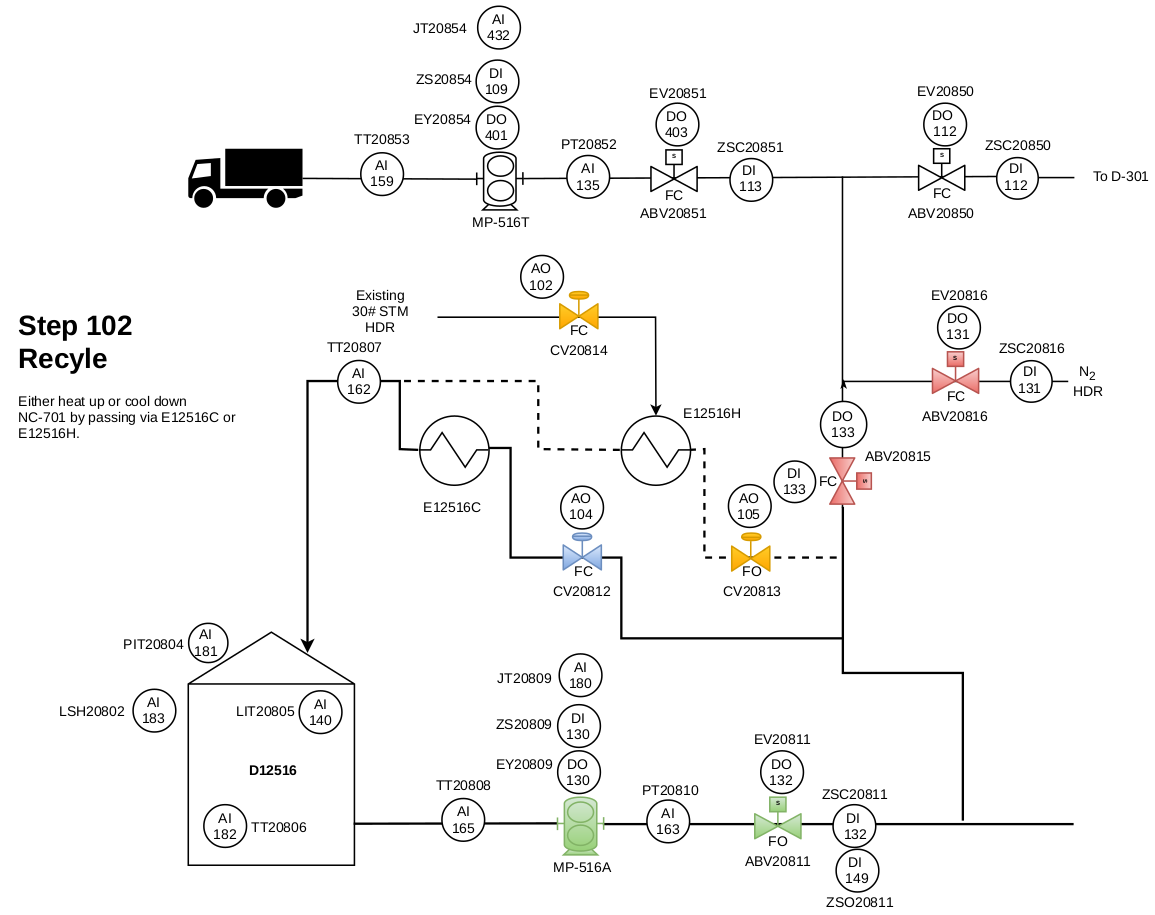
\includegraphics[angle=90,width=10cm]{/home/prasanna/Documents/git/CSR/images/Recycle.png}
\caption{Recycle step}
\end{figure}


\subsection{Transfer}
\label{sec:org0b12ac7}
\begin{figure}[htbp]
\centering
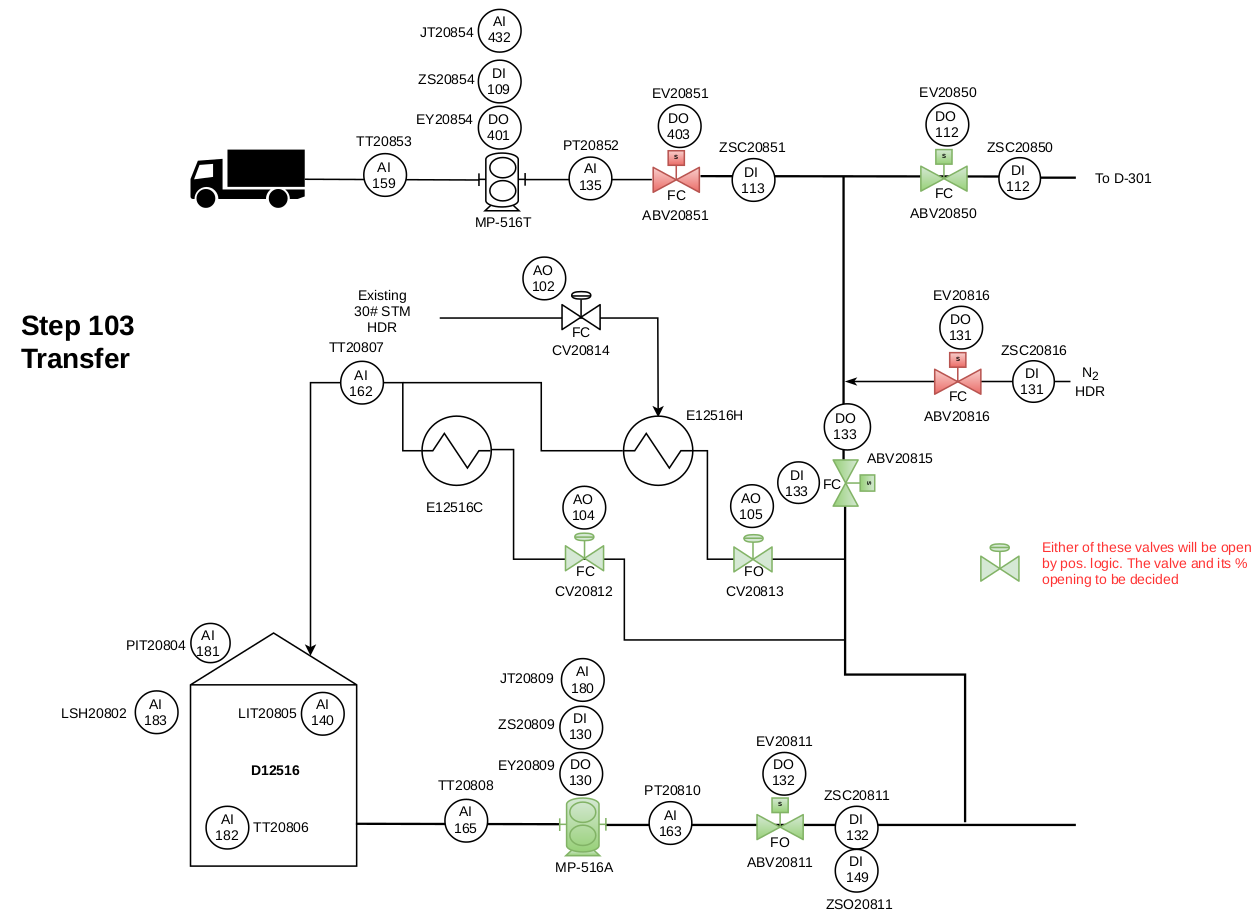
\includegraphics[angle=90,width=10cm]{/home/prasanna/Documents/git/CSR/images/Transfer.png}
\caption{Transfer from D-12516 to D-301}
\end{figure}
\subsection{Unload}
\label{sec:orge403f12}
\begin{figure}[htbp]
\centering
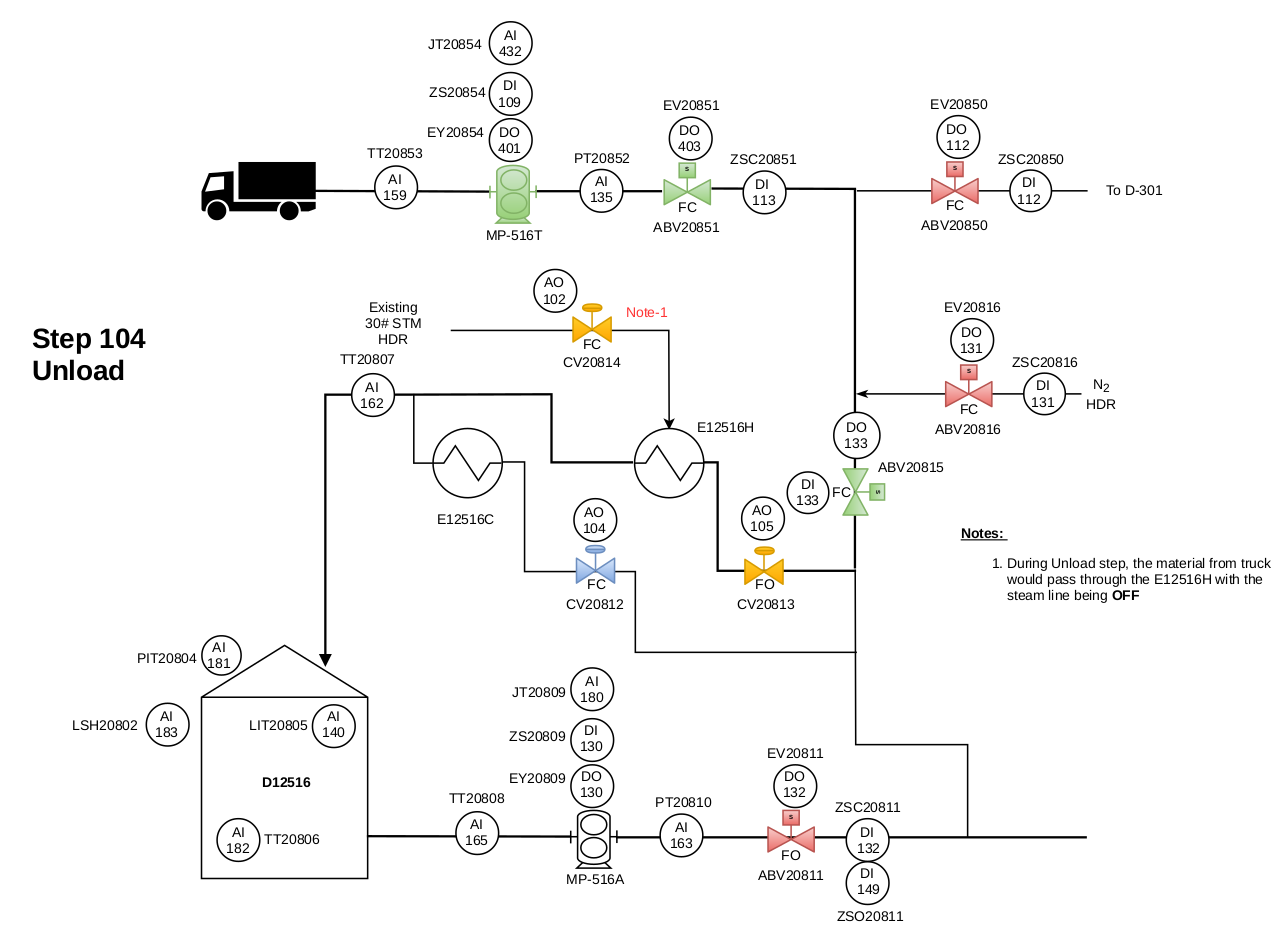
\includegraphics[angle=90,width=10cm]{/home/prasanna/Documents/git/CSR/images/Unload.png}
\caption{Unload from truck to D-12516}
\end{figure}
\subsection{Direct Transfer}
\label{sec:org41aa648}
\begin{figure}[htbp]
\centering
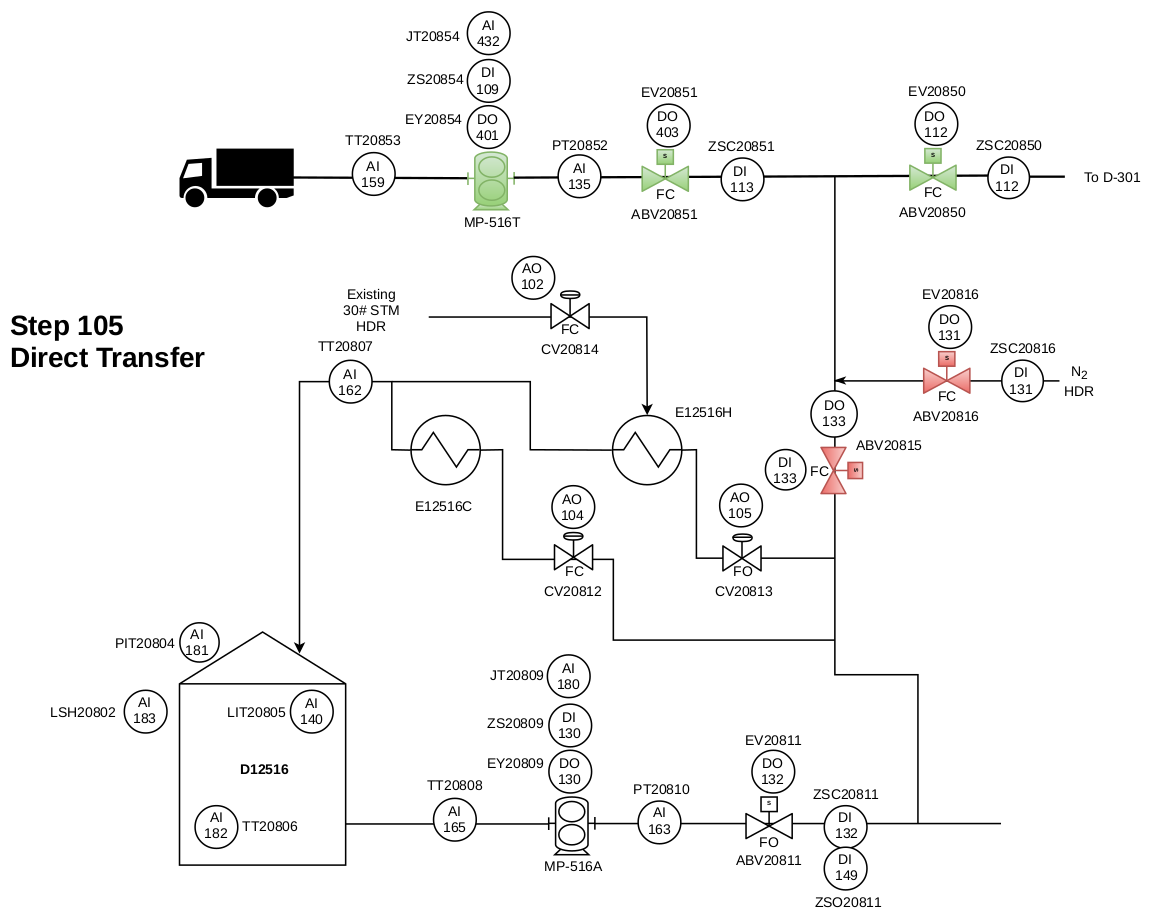
\includegraphics[angle=90,width=10cm]{/home/prasanna/Documents/git/CSR/images/DirectTransfer.png}
\caption{Unload from truck and Direct transfer to D-301}
\end{figure}
\subsection{Line Clear}
\label{sec:orga0a1ed8}
\begin{figure}[htbp]
\centering
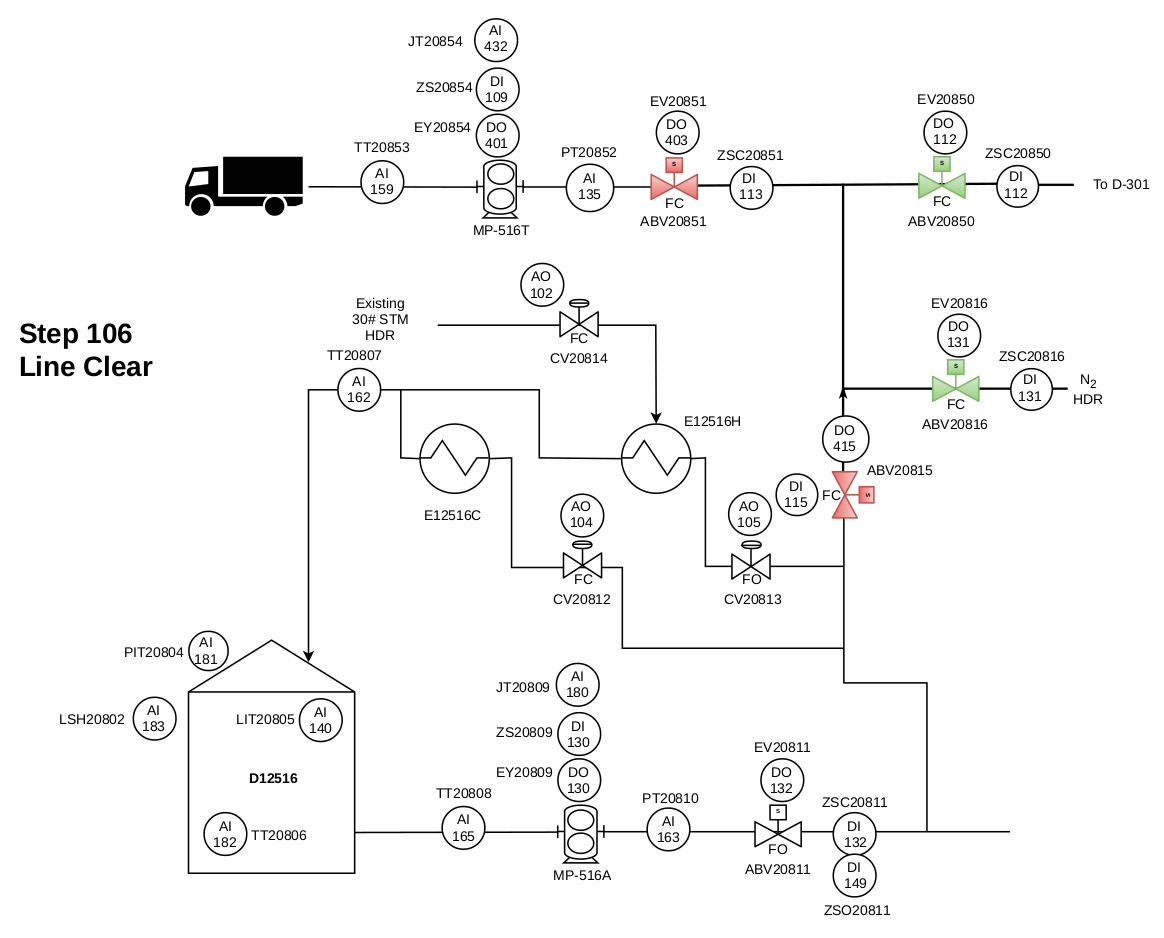
\includegraphics[angle=90,width=10cm]{/home/prasanna/Documents/git/CSR/images/LineClear.png}
\caption{Line clear}
\end{figure}
\section{Control System and IO summary}
\label{sec:org01f48c6}
Based on the proposed control narrative, the following IO count would be required to realize the project. 
\begin{center}
\begin{tabular}{rlr}
S.No. & IO Type & IO Qty\\
\hline
1 & AI & 5\\
2 & AO & 3\\
3 & DI & 8\\
4 & DO & 7\\
\end{tabular}
\end{center}

\section{Bill of Material}
\label{sec:org32c3b42}
\section{Conclusion}
\label{sec:org0cee532}
\section{References}
\label{sec:orgaf6efea}
\href{https://www.controlglobal.com/assets/knowledge\_centers/abb/assets/Benefits-of-state-based-control-white-paper.pdf}{1. Benefits of State Based Control}
\begin{enumerate}
\item 
\end{enumerate}
\end{document}
